\documentclass{scrartcl}

\usepackage[german]{babel}
\usepackage{graphicx}
\usepackage[utf8]{inputenc}
\usepackage[T1]{fontenc}
\usepackage[pdfborderstyle={/S/U/W 1}]{hyperref}
\usepackage[scaled]{helvet}
\usepackage{geometry}

\geometry{a4paper,left=30mm,right=30mm, top=3cm, bottom=3cm}

{
\titlehead{\centering
\includegraphics[width=10cm]{Logo.png}}
\title{\fontsize{40}{48} \selectfont \textsc{Implementierungsheft}\\
{\fontsize{18}{18} \selectfont Multimediatool zum Testen von Videoencodern}}}
\author {Johannes Werner, Noel Schuhmacher, Sascha Rapp,\\ Simon Grafenhorst,
Carina Weber, Jan Benedikt Schwarz}

\begin{document} {
\maketitle
\thispagestyle{empty}
\pagestyle{empty}
\newpage
\setcounter{page}{0}
\pdfbookmark{\contentsname}{toc}
\tableofcontents
\clearpage
\pagestyle{plain}
\newpage
\setcounter{page}{1}
\section{Einleitung}
In der Implementierungsphase ist es das Ziel, die Planung aus den zwei vorhergehenden Phasen in Code umzusetzen. Dieses Dokument zeigt dabei den Verlauf der Phase und entstandene Änderungen sowohl an der geplanten Funkionalität als auch am Entwurf auf.
\bigskip
\paragraph{2 Entwurfsänderungen} In diesem Kapitel werden alle Änderungen, die am Entwurf gemacht wurden, nacheinander mit einer kurzen Begründung aufgelistet. Die Klassen wurden nach Vererbunghierachien und nach Paketen in Unterkapitel sortiert, um das Auffinden einzelner Klassen zu erleichtern.
\paragraph{3 Ergebnis} Im ersten Teil dieses Kapitels wird der zeitliche Verlauf der Phase kurz dargestellt. Dannach werden alle Änderungen, die bereits im vorigen Kapitel aufgelistet wurden, auf einer gröberen Ebene dargestellt und die Gründe für die größten Änderungen erläutert. Dannach wird auf die Unterschiede zwischen den im Pflichtenheft gemachten Angaben und dem fertigen Programm eingangen. Angefangen wird mit der GUI, über weggelassene Funktionalität hin zu zusätzlich implementierter Funktionalität.
\paragraph{4 Testüberdeckung} Dieses Kapitel gibt einen kurzen Einblick in die Testüberdeckung des Codes.
\newpage
\section{Entwurfsänderungen}
\subsection{Legende}
\bigskip
\textbf{Aufbau eines Eintrags:}
\begin{verbatim}
{+,-,#} (Sichtbarkeitsbereich) ...

(optional) alter Ausdruck => neuer Ausdruck
\end{verbatim}
Grund der Änderung.\\
\\
\bigskip
\textbf{Änderungszeichen:}
\begin{itemize}
\item[] + \hspace{5mm}-->\hspace{5mm} Hinzugefügt
\item[] -  \hspace{5mm}-->\hspace{5mm} Entfernt
\item[] \# \hspace{5mm}-->\hspace{5mm} Geändert
\end{itemize}
\bigskip
\textbf{Sichtbarkeitsbereiche:}
\begin{itemize}
\item public
\item public slots
\item signals
\item protected
\item private slots
\item private
\end{itemize}
\newpage
\subsection{Allgemeines}
\bigskip
\begin{itemize}
\item Korrigierte Rechtschreibfehler in den Klassen-/Methodennamen werden nicht dokumentiert.
\item Allen Attributen wird ein Unterstrich zur bessern Lesbarkeit des Codes angehängt.
\item Gui-Klassen werden folgende Methoden bei Bedarf hinzugefügt:
\begin{verbatim}
+ (private) void createUi()
+ (private) void connectActions()
\end{verbatim}
Diese Methoden dienen allein der Lesbarkeit des Codes.
\item Änderungen an den folgenden Methodenspezifizierern werden nicht dokumentiert:
\begin{verbatim}
const
noexcept
\end{verbatim}
\item Destruktoren werden in allen Klassen als implzit gegeben betrachtet und bei Bedarf implementiert.
\end{itemize}
\newpage
\subsection{Entfernte Klassen}
\bigskip
\subsubsection{ApplyFilter}
Wurde entfernt, da das Anwenden der Filter nicht Rückgängig gemacht werden kann.
\subsubsection{BlendingFilter}
Wurde entfernt, da der Filter im Konflikt mit der Filtervorschau Funktionalität stand.
\subsubsection{ZoomFilter}
Wurde entfernt, da ein Bug in libavfilter auftrat, aufgrunddessen das Bild falsch skaliet wurde.
\bigskip
\subsection{Umbenannte Klassen}
\bigskip
\subsubsection{BlackWhiteFilter}
Wurde umbenannt in GrayscaleFilter.\\
Korrekte Übersetzung ins Englische.
\newpage
\subsection{Hinzugefügte Klassen}
\bigskip
\subsubsection{ChangeFilter}
War implementierungstechnisch kein Mehraufwand.
\subsubsection{GraphVideo}
Um Rgb Histogramme für Videos anzeigen zu können.
\subsubsection{ResultSaver}
Trennen vom Speichern des Projektes und der Ergebnisse.
\subsubsection{VideoSaver}
Um encodierte Videos speichern zu können.
\subsubsection{AnalysisGraph}
Enum für bessere Schnittstelle.
\subsubsection{AnalysisVideo}
Enum für bessere Schnittstelle.
\subsubsection{GraphCalculator}
Um das Berrechnen vom Anzeigen zu trennen.
\subsubsection{GraphPlayer}
Um Rgb Histogramme abspielen zu können.
\newpage
\subsection{Filterkofigurationsboxen}
\subsubsection{Basisklasse: FilterConfigurationBox}
\bigskip
\begin{verbatim}
+ (public) static std::unique_ptr<FilterConfigurationBox>
CreateConfigurationBox(FilterTab& filterTab, Model::Filter& filter)
\end{verbatim}
Fabrikmethode zur Erstellung einer FilterConfigurationBox für einen bestimmten Filter.
\bigskip
\begin{verbatim}
+ (public) void setFilterTab(FilterTab& filterTab)
+ (public) void setFilterIndex(std::size_t index)
+ (private) std::size_t index
+ (private) FilterTab* filterTab
\end{verbatim}
Dass der UndoCommand zum Rückgaengig machen der Änderung am Filter korrekt erstellt werden kann.
\bigskip
\begin{verbatim}
+ (public) virtaul void updateUi()
\end{verbatim}
Um der FilterConfigurationBox bescheid sagen zu können, dass der Filter sich ausserhalb der Box geändert hat.
\bigskip
\begin{verbatim}
+ (protected) void updatePreview()
\end{verbatim}
Wird von der erbenden Klasse aufgerufen, um die Vorschau entsprechend den Änderungen des Benutzers anzupassen.
\bigskip
\begin{verbatim}
+ (protected) void updateTempFilter();
\end{verbatim}
Wird von der erbenden Klasse aufgerufen, um den temporären Filter auf den Stand des originalen Filters zu bringen.
\bigskip
\begin{verbatim}
+ (private slots) applyFilter()
+ (private slots) resetFilter()
\end{verbatim}
Slots für die entsprechenden Buttons.
\bigskip
\begin{verbatim}
+ (private) static QImage& getDefaultImage()
+ (private) static std::unique_ptr<QImage> defaultImage
\end{verbatim}
Stellt das Standardbild für die Vorschau zur Verfuegung.
\bigskip
\begin{verbatim}
+ (protected) std::unique_ptr<Model::Filter> tempFilter
\end{verbatim}
Temporäres Filterobjekt, auf welches die erbende Klasse die Änderungen des Benutzers anwendet.
\bigskip
\begin{verbatim}
+ (protected) QScrollArea* filterOptionsArea
+ (private) std::unique_ptr<QImage>
+ (private) FrameView* filterPreview
+ (private) QLabel* label_filter
+ (private) QPushButton* button_apply
+ (private) QPushButton* button_reset
\end{verbatim}
Steuerung der Gui.
\bigskip
\subsubsection{Allgemein erbende Klassen}
\bigskip
\begin{verbatim}
+ (protected) void updateUi()
\end{verbatim}
Geerbt aus der Basisklasse.
\bigskip
\begin{verbatim}
+ (private) void createFilterOptions()
\end{verbatim}
Erstellt die Gui.
\bigskip
\begin{verbatim}
+ (private slots) ...
\end{verbatim}
Slots fuer die Gui-Elemente.
\bigskip
\begin{verbatim}
+ (private) ...
\end{verbatim}
Attribute zur Steuerung der Gui.
\newpage
\subsection{Filter}
\subsubsection{Basisklasse: Filter}
\bigskip
\begin{verbatim}
+ (public) static std::unique_ptr<Filter> CreateFilter(QString filtername)
\end{verbatim}
Fabrikmethode um einen Filter aufgrund des Namens zu erstellen.
\bigskip
\begin{verbatim}
# (public) virtual std::string getName()

std::string => QString
\end{verbatim}
Bessere Kompatibilität mit den Qt Gui Elementen.
\bigskip
\begin{verbatim}
+ (public) virtual void restore(QString description)
+ (public) virtual QString getSaveString()
\end{verbatim}
Zum einfachen Kopieren von Filtern, wenn die konkrete Klasse nicht bekannt ist und zum einfachen Laden und Speichern der Filter.
\bigskip
\subsubsection{Allgemein erbende Klassen}
\begin{verbatim}
+ (public) static const QString FILTERNAME
\end{verbatim}
Um Filternamen nicht 'nackt' in den Quelltext zu schreiben.
\bigskip
\begin{verbatim}
+ (public) void QString getName()
+ (public) void restore(QString description)
+ (public) void QString getSaveString()
\end{verbatim}
Geerbt aus der Basisklasse. 
\newpage
\subsubsection{BlurFilter}
\bigskip
\begin{verbatim}
- (public) bool getPreserveEdges()
- (public) bool setPreserveEdges()
- (private) bool preserveEdges
\end{verbatim}
Die Option hatte keinen Effekt auf das Ergebnis.
\bigskip
\subsubsection{BorderFilter}
\bigskip
\begin{verbatim}
# (public) void setColor(QRgb color)
# (public) QRgb getColor()
# (private) QRgb color

QRgb => QColor
\end{verbatim}
Komfortablerer Umgang mit QColor.
\bigskip
\subsubsection{GridFilter}
\bigskip
\begin{verbatim}
# (public) void setColor(QRgb color)
# (public) QRgb getColor()
# (private) QRgb color

QRgb => QColor
\end{verbatim}
Komfortablerer Umgang mit QColor.
\bigskip
\subsubsection{RectangleFilter}
\bigskip
\begin{verbatim}
# (public) void setColor(QRgb color)
# (public) QRgb getColor()
# (private) QRgb color

QRgb => QColor
\end{verbatim}
Komfortablerer Umgang mit QColor.
\newpage
\subsection{Mementos}
\subsubsection{AnalysisBoxContainerMemento}
\bigskip
\begin{verbatim}
# (public) std::vector<AnalysisBoxMemento> getAnalysisBoxList()

std::vector<AnalysisBoxMemento> 
=> std::vector<std::unique_ptr<AnalysisBoxMemento>>&

# (private) std::vector<AnalysisBoxMemento*> mementoList

std::vector<AnalysisBoxMemento*>
=>std::vector<std::unique_ptr<AnalysisBoxMemento>>
\end{verbatim}
Unnötiges Kopieren vermeiden und nackte Pointer vermeiden.
\bigskip
\begin{verbatim}
- (public) void setAnalysisBoxList(std::vector<AnalysisBoxMemento> analysisBoxList)
+ (public) void addMemento(std::unique_ptr<AnalysisBoxMemento> memento)
\end{verbatim}
Komfortablere Schnittstelle.
\bigskip
\subsubsection{AnalysisBoxMemento}
\bigskip
\begin{verbatim}
# (public) QString getVideoPath()
# (public) void setVideoPath(QString videoPath)
# (private) QString videoPath

VideoPath => Path

# (public) Model::Video* getMacroVideo()
# (public) void setMacroVideo(Model::Video* macroVideo)
# (private) Model::Video* macroVideo

Macro => MacroBlock

# (public) Model::Graph getPsnr()
# (public) void setPsnr(Model::Graph psnr)
# (private) Model::Graph psnr

Psnr => PsnrGraph

# (public) Model::Graph getBitrate()
# (public) void setBitrate(Model::Graph Bitrate)
# (private) Model::Graph bitrate

bitrate => bitrateGraph
\end{verbatim}
Sauberere Namensgebung.
\newpage
\begin{verbatim}
# (public) Model::Graph getPsnrGraph()
# (public) void setPsnrGraph(Model::Graph psnr)
# (private) Model::Graph psnrGraph
# (public) Model::Graph getBitrateGraph()
# (public) void setBitrateGraph(Model::Graph bitrate)
# (private) Model::Graph bitrateGraph

Model::Graph => Model::Graph*
\end{verbatim}
Unnötiges Kopieren vermeiden.
\bigskip
\begin{verbatim}
+ (public) void setEncoder(QString encoder)
+ (public) QString getEncoder()
+ (public) void setAverageBitrate(QString bitrate)
+ (public) QString getAverageBitrate()
+ (public) void setFilename(QString filename)
+ (public) QString getFilename()
+ (public) void setFilesize(QString size)
+ (public) QString getFilesize()
+ (public) void setRedHistogram(Model::GraphVideo* video)
+ (public) Model::GraphVideo* getRedHistogram()
+ (public) void setGreenHistogram(Model::GraphVideo* video)
+ (public) Model::GraphVideo* getGreenHistogram()
+ (public) void setBlueHistogram(Model::GraphVideo* video)
+ (public) Model::GraphVideo* getBlueHistogram()

+ (private) QString encoder
+ (private) QString avergaeBitrate
+ (private) QString filename
+ (private) QString filesize
+ (private) Model::GraphVideo* redHistogram
+ (private) Model::GraphVideo* greenHistogram
+ (private) Model::GraphVideo* blueHistogram
\end{verbatim}
Vergessene Attribute, die auch gespeichert werden müssen.
\newpage
\subsubsection{AnalysisTabMemento}
\bigskip
\begin{verbatim}
# (public) int getCurrentVideoPosition()
# (public) void setCurrentVideoPosition(int currentVideoPosition)
# (private) int currentVideoPosition

CurrentVideo => Player
\end{verbatim}
Sauberere Namensgebung.
\bigskip
\begin{verbatim}
- (public) int getCurrentlyShownAnalysisVideo()
- (public) void setCurrentlyShownAnalysisVideo(int currentVideo)
- (private) int currentlyShownAnalysisVideo
- (public) float getCurrentSpeed()
- (public) void setCurrentSpeed(float currentSpeed)
- (private) currentSpeed
\end{verbatim}
Nicht realisierbar bzw. nicht mehr von nöten.
\bigskip
\begin{verbatim}
# (public) AnalysisBoxContainerMemento getAnalysisBoxContainerMemento()

AnalysisBoxContainerMemento => AnalysisBoxContainerMemento*

# (public) void setAnalysisBoxContainerMemento(AnalysisBoxContainerMemento memento)

AnalysisBoxContainerMemento => std::unique_ptr<AnalysisBoxContainerMemento>

+ (private) std::unique_ptr<AnalysisBoxContainerMemento> analysisboxMemento
\end{verbatim}
Unnötiges Kopieren vermeiden.
\bigskip
\begin{verbatim}
+ (public) void setRawVideo(Model::YuvVideo* video)
+ (public) void setRawVideo(std::unique_ptr<Model::YuvVideo> video)
+ (public) std::unique_ptr<Model::YuvVideo> releaseVideo()
+ (public) Model::YuvVideo* getRawVideo()
+ (public) GUI::AnalysisGraph getAnalysisGraph()
+ (public) void setAnalysisGraph(GUI::AnalysisGraph graph)
+ (public) GUI::AnalysisVideo getAnalysisVideo()
+ (public) void setAnalysisVideo(GUI::AnalysisVideo video)
+ (private) Model::YuvVideo* rawVideo
+ (private) std::unique_ptr<Model::YuvVideo> ownedVideo
+ (private) GUI::AnalysisGraph graph
+ (private) GUI::AnalysisVideo video
\end{verbatim}
Vergessene Attribute, die auch gespeichert werden müssen.
\newpage
\subsubsection{FilterTabMemento}
\bigskip
\begin{verbatim}
# (public) bool getWasApplied()
# (public) void setWasApplied(bool wasApplied)
# (private) bool wasApplied

WasApplied => IsFilteredVideoShown

# (public) int getDisplayedFrame()
# (public) void setDisplayedFrame(int displayedFrame)
# (private) int displayedFrame

DisplayedFrame => CurrentFrame
\end{verbatim}
Sauberere Namensgebung.
\bigskip
\begin{verbatim}
# (public) Model::FilterList getFilterList()
# (public) void setFilterList(Model::FilterList list)
# (private) Model::FilterList  filterList

Model::FilterList => std::unique_ptr<Model::FilterList>
\end{verbatim}
Abstrakte Klassen können nur als Pointer übergeben werden.
\bigskip
\begin{verbatim}
- (public) std::string getLoadedFile()
- (public) void setLoadedFile(std::string loadedFile)
- (private) std::string loadedFile
\end{verbatim}
Wurden ersetzt durch bessere Methoden.
\bigskip
\begin{verbatim}
+ (public) void setRawVideo(Model::YuvVideo* rawVideo)
+ (public) void setRawVideo(std::unique_ptr<Model::YuvVideo> video)
+ (public) std::unique_ptr<Model::YuvVideo> releaseVideo()
+ (public) Model::YuvVideo* getRawVideo()
+ (public) void setIsPreviewShown(bool isShown)
+ (public) bool isPreviewShow()
+ (public) void setCurrentFrame(int currentFrame)
+ (public) int getCurrentFrame()
+ (public) void setCurrentlySelectedFilter(int filter)
+ (public) int getCurrentlySelectedFilter()
+ (private) Model::YuvVideo* rawVideo
+ (private) std::unique_ptr<Model::YuvVideo> ownedRawVideo
+ (private) bool isPreviewShown
+ (private) int currentFrame
+ (private) int currentlySelectedFilter
\end{verbatim}
Vergessene Attribute, die auch gespeichert werden müssen.
\newpage
\subsubsection{MainWindowMemento}
\bigskip
\begin{verbatim}
# (public) AnalysisTabMemento getAnalysisTabMemento()
# (public) FilterTabMemento getFilterTabMemento()

AnalysisTabMemento => AnalysisTabMemento*
FilterTabMemento => FilterTabMemento*

# (public) void setAnalysisTabMemento(AnalysisTabMemento memento)
# (public) void setFilterTabMemento(FilterTabMemento memento)

AnalysisTabMemento => std::unique_ptr<AnalysisTabMemento>
FilterTabMemento => std::unique_ptr<FilterTabMemento>

# (private) AnalysisTabMemento* analysisTab
# (private) FilterTabMemento* filterTab

AnalysisTabMemento* => std::unique_ptr<AnalysisTabMemento>
FilterTabMemento* => std::unique_ptr<FilterTabMemento>
\end{verbatim}
Unnötiges Kopieren und nackte Pointer vermeiden.
\newpage
\subsection{Undo Commands}
\subsubsection{AddFilter}
\begin{verbatim}
# (public) AddFilter(GUI::FilterTab* filterTab,Model::Filter filter)

(...) => (GUI::FilterTab& filterTab, QString filternam)

- (private) Model::Filter filter
+ (private) QString filtername
+ (private) std::unique_ptr<Memento::FilterTabMemento> memento
\end{verbatim}
Benötigte Attribute zum Rückgängig machen haben sich geändert.
\bigskip
\subsubsection{AddVideo}
\begin{verbatim}
# (public) AddVideo(GUI::AnalysisBoxContainer* container,Model::EncodedVideo video)

Model::EncodedVideo => QString

- (private) Model::EncodedVideo video
+ (private) QString filename
\end{verbatim}
Benötigte Attribute zum Rückgängig machen haben sich geändert.
\bigskip
\subsubsection{FilterReset}
\begin{verbatim}
# (public) FilterReset(GUI::FilterTab* tab,Model::FilterList list)

(...) => (GUI::FilterTab& filterTab)

# (private) Model::FilterList filterList

Model::FilterList => std::unique_ptr<Model::FilterList>

+ (private) std::unique_ptr<Memento::FilterTabMemento> memento
\end{verbatim}
Benötigte Attribute zum Rückgängig machen haben sich geändert.
\newpage
\subsubsection{LoadAnalysisVideo}
\begin{verbatim}
# (public) LoadAnalysisVideo(GUI::AnalysisTab* tab, 
Memento::AnalysisTabMemento memento, Model::YuvVideo video)

(...) => (GUI::AnalysisTab* tab, std::unique_ptr<YuvVideo> video)

# (private) Model::YuvVideo* video

Model::YuvVideo* => std::unique_ptr<YuvVideo>

+ (private) std::unique_ptr<Memento::AnalysisTabMemento> memento
\end{verbatim}
Benötigte Attribute zum Rückgängig machen haben sich geändert.
\bigskip
\subsubsection{LoadFilterConfig}
\begin{verbatim}
# (public) LoadFilterConfig(GUI::FilterTab* tab,
Model::FilterList old,Model::FilterList new)

(...) => (GUI::FilterTab& tab,std::unique_ptr<Model::FilterList> newList)

# (private) Model::Filter:ist* newList

Model::FilterList* => std::unique_ptr<Model::FilterList>

- (private) Model::FilterList* oldList
+ (private) std::unique_ptr<Memento::FilterTabMemento> memento
\end{verbatim}
Benötigte Attribute zum Rückgängig machen haben sich geändert.
\bigskip
\subsubsection{LoadFilterVideo}
\begin{verbatim}
# (public) LoadFilterVideo(GUI::FilterTab* tab,Model::YuvVideo video,
Memento::FilterTabMemento memento)

(...) => (GUI::FilterTab& tab,std::unique_ptr<Model::YuvVideo> video,
std::unique_ptr<Memento::FilterTabMemento> memento)

# (private) Memento::FilterTabMemento* memento
# (private) Model::YuvVideo* video

Memento::FilterTabMemento* => std::unique_ptr<FilterTabMemento>
Model::YuvVideo* => std::unique_ptr<Model::YuvVideo>
\end{verbatim}
Benötigte Attribute zum Rückgängig machen haben sich geändert.
\newpage
\subsubsection{MoveFilterDown}
\begin{verbatim}
# (public) MoveFilterDown(GUI::FilterTab* tab, int oldIndex, int newIndex)

(...) => (GUI::FilterTab& tab, int index)

- (private) int newIndex
- (private) int oldIndex
+ (private) int index
+ (private) std::unique_ptr<Memento::FilterTabMemento>
\end{verbatim}
Benötigte Attribute zum Rückgängig machen haben sich geändert.
\bigskip
\subsubsection{MoveFilterUp}
Genau diesselben Aenderungen wie in der Klasse 'MoveFilterDown'.
\subsubsection{RemoveFilter}
\begin{verbatim}
# (public) RemoveFilter(GUI::FilterTab* tab,Model::Filter filter, int index)

(...) => (GUI::FilterTab& tab, int index)

# (private) Model::Filter* filter

Model::Filter* => std::unique_ptr<Model::filter>

+ (private) std::unique_ptr<Memento::FilterTabMemento> memento
\end{verbatim}
Benötigte Attribute zum Rückgängig machen haben sich geändert.
\bigskip
\subsubsection{RemoveVideo}
\begin{verbatim}
# (public) RemoveVideo(GUI::AnalysisBoxContainer* container, Model::EncodedVideo video)

(...) => (GUI::AnalysisBoxContainer* container, GUI::AnalysisBox* box)

- (private) Model::EncodedVideo* video
+ (private) int index
+ (private) std::unique_ptr<Memento::AnalysisBoxMemento> memento
\end{verbatim}
Benötigte Attribute zum Rückgängig machen haben sich geändert.
\newpage
\subsubsection{WriteComment}
\begin{verbatim}
# (public) WriteComment()

() => (GUI::AnalysisBoxContainer* container, int index, QString oldComment,
QString newComment)

+ (private) GUI::AnalysisBoxContainer* container
+ (private) int index
+ (private) QString oldComment
+ (private) QString newComment
\end{verbatim}
Benötigte Attribute zum Rückgängig machen haben sich geändert.
\newpage
\subsection{Model}
\subsubsection{AVVideo}
\bigskip
\begin{verbatim}
std::unique_ptr<AVFrame> => AVFrame*
int index => std::size_t index
\end{verbatim}
Änderungen aufgrund der Implementierung von AVFrame und std::vector.
\bigskip
\begin{verbatim}
# (public) AVVideo(int fps, int width, int height)

(...) => (int fps)
\end{verbatim}
Die Dimension wird jetzt vom ersten Frame, dass in das Video gesteckt wird, bestimmt.
\bigskip
\begin{verbatim}
- (public) void insertFrames(int index, std::vector<std::unique_ptr<AVFrame>>& frames)
\end{verbatim}
Wird nicht benötigt.
\bigskip
\begin{verbatim}
+ (public) void setFps(int fps)
\end{verbatim}
Um beim Konvertieren die Fps korrekt zu setzen.
\bigskip
\begin{verbatim}
+ (public) void appendFrame(AVFrame* frame)
\end{verbatim}
Komfortablere Schnittstelle.
\bigskip
\begin{verbatim}
+ (public) bool isComplete()
+ (public) void setIsComplete(bool isComplete)
+ (private) bool isComplete
\end{verbatim}
Um feststellen zu können, ob das Video vollständig ist, oder noch auf Frames gewartet werden muss.
\newpage
\subsubsection{EncodedVideo}
\bigskip
\begin{verbatim}
- (public) int getFileSize()
- (public) getNumberOfColors()
- (public) void setBitrate (Model::Graph graph)
- (public) void setPsnr (Model::Graph graph)
- (public) void setRedHistogramm (Model::Graph graph)
- (public) void setGreenHistogramm (Model::Graph graph)
- (public) void setBlueHistogramm (Model::Graph graph)
- (public) void setMacroblockVideo (GUI::Video video)
- (public) void setRgbDiffVideo (GUI::Video video)
- (private) int fileSize
- (private) int numberOfColors
- (private) QString codec
\end{verbatim}
Wird nicht benötigt.
\bigskip
\begin{verbatim}
# (public) Model::Graph& getRedHistogram()
# (public) Model::Graph& getGreenHistogram()
# (public) Model::Graph& getBlueHistogram()
# (private) Model::Graph* redHisto
# (private) Model::Graph* greenHisto
# (private) Model::Graph* blueHisto

Model::Graph& => Model::GraphVideo&
Model::Graph* => std::unique_ptr<Model::GraphVideo>
\end{verbatim}
Um Rgb Histogramme für das Video speichern zu können.
\bigskip
\begin{verbatim}
# (public) Model::Graph& getPsnr()

Model::Graph& => Model::Graph*
() => (Model::Video* reference)

# (public) Model::Video& getRgbDiffVideo(Model::Video* reference)

Model::Video& => Model::Video*
\end{verbatim}
Wenn die reference null ist und nicht berechnet werden kann, muss ein nullptr zurück gegeben werden.
\bigskip
\begin{verbatim}
+ (public) int getAverageBitrate()
\end{verbatim}
Zusätzliches Attribut zum Anzeigen.
\newpage
\begin{verbatim}
# (private) Model::Video* video
# (private) Model::AVVideo* avVideo
# (private) Model::Video* rgbDiffVideo
# (private) Model::Video* macroBlockVideo
# (private) Model::Graph* bitrate
# (private) Model::Graph* psnr

Model::Video* => std::unique_ptr<Model::Video>
Model::AVVideo* => std::unique_ptr<Model::AVVideo>
Model::Graph* => std::unique_ptr<Model::Graph>

- (private) Model::Video* displayVideo
\end{verbatim}
Nackte Pointer vermeiden.
\bigskip
\begin{verbatim}
+ (private) std::unique_ptr<Utility::VideoLoader> loader
+ (private) 	std::unique_ptr<Utility::BitrateCalculator> bitrateCalculator
+ (private) std::unique_ptr<Utility::RGBHistogramCalculator> rgbHistoCalculator
+ (private) std::unique_ptr<Utility::PsnrCalculator> psnrCalculator
+ (private) std::unique_ptr<Utility::RGBDifferenceCalculator> rgbDiffCalculator
+ (private) std::unique_ptr<Utility::VideoConverter> macroblockConverter
+ (private) std::unique_ptr<Utility::VideoConverter> videoConverter
+ (private) std::unique_ptr<Utility::VideoLoader> macroblockLoader
+ (private) void calculateHistograms()
\end{verbatim}
Attribute zur Berrechnung der einzelnen Videos und Graphen.
\newpage
\subsubsection{FilterList}
\bigskip
\begin{verbatim}
- (public) Filter* getFilterByName(std::string name)
- (public) int getIndex(std::string name)
- (public) void addFilter(std::string name, int index)
- (public) void removeFilter(std::string name)
\end{verbatim}
Schlechte Schnittstelle.
\bigskip
\begin{verbatim}
+ (public) std::unique_ptr<Filter> removeFilter(std::size_t index)
+ (public) Filter* appendFilter(QString name)
+ (public) void insertFilter(std::unique_ptr<Filter> filter, std::size_t index)
+ (public) std::size_t getSize()

# (public) void moveFilter(int oldPos, int newPos)

int => std::size_t
\end{verbatim}
Bessere Schnittstelle.
\bigskip
\begin{verbatim}
# (private) std::vector<Filter*> filters

Filter => std::unique_ptr<Filter>
\end{verbatim}
Nackt Pointer vermeiden.
\bigskip
\subsubsection{Graph}
\bigskip
\begin{verbatim}
- (public) void cut(int x)
\end{verbatim}
Wird nicht benötigt.
\bigskip
\begin{verbatim}
# (public) void addValue(int x, double y)
# (public) double getValue(int x)
# (public) removeValue(int x)
# (public) int getLength()

addValue => setValue
getLength => getSize
int => std::size_t

+ (public) getBiggestValue()
\end{verbatim}
Bessere Schnittstelle.
\newpage
\subsubsection{Project}
\bigskip
\begin{verbatim}
# (public) void setMemento(Memento::MainWindowMemento memento)
# (private) Memento::MainWindowMemento* memento

Memento::MainWindoeMemento => std::unique_ptr<Memento::MainWindowMemento>
Memento::MainWindoeMemento* => std::unique_ptr<Memento::MainWindowMemento>
\end{verbatim}
Unnötiges Kopieren vermeiden.
\bigskip
\begin{verbatim}
+ (public) void setName(QString name)
\end{verbatim}
Um den Namen des Projektes setzen zu können, welches beim Start des Programms als leeres Projekt erstellt wird.
\bigskip
\subsubsection{Video}
\bigskip
\begin{verbatim}
# (public) Video(int fps, int width, int height)

(...) => (int fps)
\end{verbatim}
Die Dimension wird jetzt vom ersten Frame, dass in das Video gesteckt wird, bestimmt.
\bigskip
\begin{verbatim}
- (public) void insertFrames(int index, std::vector<std::unique_ptr<QImage>>& frames)
\end{verbatim}
Wird nicht benötigt.
\bigskip
\begin{verbatim}
# (public) QImage* getFrame(int index)
# (public) void insertFrame(std::unique_ptr<QImage> frame, int index)
# (public) void removeFrame(int index)
# (public) int getNumberOfFrames()

int => std::size_t
\end{verbatim}
An die Schnittstelle von vector anpassen.
\bigskip
\begin{verbatim}
+ (public) void setFps(int fps)
+ (public) bool appendFrame(std::unique_ptr<QImage> frame)
\end{verbatim}
Schnittstelle erweitern.
\bigskip
\begin{verbatim}
+ (public) void setIsComplete(bool isComplete)
+ (public) bool isComplete()
+ (private) bool isComplete
\end{verbatim}
Um feststellen zu können, ob das Video vollständig ist, oder noch auf Frames gewartet werden muss.
\newpage
\subsubsection{YuvVideo}
\bigskip
\begin{verbatim}
# (public) YuvVideo(QString path,Utility::PixelSheme type, int width, int height, int fps)

(...) => (QString path, Utility::YuvType type, 
Utility::Compression compression, int width, int height, int fps)

# (private) Utility::PixelSheme yuvType

Utility::PixelSheme => Utility::YuvType
\end{verbatim}
Compression wurde im Design vergessen und Pixelsheme und YuvType waren diesselben Klassen.
\bigskip
\begin{verbatim}
+ (public) int getWidth()
+ (public) int getHeight()
+ (public) int getFps()
\end{verbatim}
Getter wurden im Design vergessen.
\bigskip
\begin{verbatim}
+ (public) GraphVideo& getRedHistogram()
+ (public) GraphVideo& getGreenHistogram()
+ (public) GraphVideo& getBlueHistogram()
+ (private) std::unique_ptr<GraphVideo> redHisto
+ (private) std::unique_ptr<GraphVideo> greenHisto
+ (private) std::unique_ptr<GraphVideo> blueHisto
+ (private) std::unique_ptr<Utility::RGBHistogramCalculator> histogramCalculator
+ (private) void calculateHistograms();
\end{verbatim}
Zum Berrechnen von den Histogrammen.
\bigskip
\begin{verbatim}
- (public) Model::AVVideo& getAvVideo()
- (private) std::unique_ptr<Model::AVVideo> avVideo
\end{verbatim}
Wird nicht benötigt.
\bigskip
\begin{verbatim}
+ (private) std::unique_ptr<Utility::YuvFileReader> fileReader
+ (private) void loadVideo()
\end{verbatim}
Zum Laden des Videos.
\newpage
\subsection{Utility}
\subsubsection{BitrateCalculator}
\begin{verbatim}
- (public) Model::Graph calculate()
+ (public) void calculate(Model::Graph* target)

+ (private) std::thread calculator
+ (private) bool isRunning
+ (private) Model::Graph* target
+ (private) void calculateP()
\end{verbatim}
Threading.
\subsubsection{FilterApplier}
\begin{verbatim}
# (public) FilterApplier(Model::FilterList& list)

(...) => (Model::FilterList& list, int width, int height, int pixelFormat)
\end{verbatim}
Mehr informationen für Ffmpeg benötigt.
\bigskip
\begin{verbatim}
# (public) void applyToVideo(Model::AVVideo& target, Model::AVVideo& source)

Model::AVVideo => Model::Video

+ (public) void applyToVideo(Model::Video& target, Model::AVVideo& source)

- (private) AVFrame applyToFrame(AVFrame& source)
+ (public) AVFrame* applyToFrame(AVFrame& source)
\end{verbatim}
Bessere Schnittstelle.
\bigskip
\begin{verbatim}
+ (signals) void applyComplete(bool successful)
\end{verbatim}
Um die stausbar updaten zu können.
\bigskip
\begin{verbatim}
+ (private) int width
+ (private) int height
+ (private) int pixelFormat
+ (private) AVFilterGraph* filterGraph
+ (private) AVFilterContext* buffersinkContext
+ (private) AVFilterContext* buffersourceContext
+ (private) std::string filterDescription
+ (private) std::thread applier
+ (private) Model::Video* source
+ (private) Model::AVVideo* source1
+ (private) Model::Video* target
+ (private) bool isRunning
+ (private) void createFilterString()
+ (private) void applyToVideoP()
+ (private) void applyToAVVideoP()
\end{verbatim}
Threading und Attribute für Ffmpeg.
\newpage
\subsubsection{FilterConfigurationLoader}
\begin{verbatim}
# (public) Model::FilterList getConfiguratin()

Model::FilterList => std::unique_ptr<Model::FilterList>
\end{verbatim}
Unnötiges Kopieren vermeiden.
\bigskip
\subsubsection{FilterConfigurationSaver}
\begin{verbatim}
+ (private) Model::FilterList* filterList
\end{verbatim}
Speichern der Liste, die im Konstruktor übergeben wird.
\bigskip
\subsubsection{ProjectReader}
\bigskip
\begin{verbatim}
# (public) Model::Project readProject()

Model::Project => std::unique_ptr<Model::Project>
\end{verbatim}
Unnötiges Kopieren vermeiden.
\bigskip
\begin{verbatim}
+ (private) QFile file
+ (private) QTextStream dataStream

+ (private) void parseFilterTab(Memento::FilterTabMemento* memento,QString line)
+ (private) void parseAnalysisTab(Memento::AnalysisTabMemento* memento,QString line)
\end{verbatim}
Mehr Lesbarkeit des Codes.
\bigskip
\subsubsection{ProjectWriter}
\bigskip
\begin{verbatim}
# (public) ProjectWriter(Model::Project project)

Model::Project => Model::Project*
\end{verbatim}
Unnötiges Kopieren vermeiden.
\bigskip
\begin{verbatim}
- (public) void saveResults()
\end{verbatim}
Wurde in eigene Klasse ausgelagert.
\begin{verbatim}
+ (private) Model::Project* project
+ (private) std::unique_ptr<QFile> file
+ (private) QTextStream dataStream
\end{verbatim}
Attribute zum Speichern benötigt.
\newpage
\subsubsection{PsnrCalculator}
\bigskip
\begin{verbatim}
# (public) PsnrCalculator(Model::AVVideo& reference, Model::AVVideo& video)

Model::AVVideo => Model::Video
\end{verbatim}
Bessere Schnittstelle.
\begin{verbatim}
+ (private) double calculateMeanSquareError(QImage* frame1, QImage* frame2);
\end{verbatim}
Wird zum Berrechen benötigt.
\bigskip
\begin{verbatim}
+ (private) std::thread calculator
+ (private) Model::Graph* target
+ (private) bool isRunning

+ (private) void calculateP()
\end{verbatim}
Threading.
\bigskip
\subsubsection{RgbDifferenceCalculator}
\begin{verbatim}
# (public) void calculateVideo(Model::Video& target)

Model::Video& => Model::Video*
\end{verbatim}
Bessere Schnittstelle.
\bigskip
\begin{verbatim}
+ (private) Model::Video* target
+ (private) std::thread calculator
+ (private) bool isRunning

+ (private) void calculateP()
\end{verbatim}
Threading.
\newpage
\subsubsection{RGBHistogramCalculator}
\begin{verbatim}
# (public) void calculate()

() => (Model::GraphVideo* targetRed,Model::GraphVideo* targetGreen, 
Model::GraphVideo* targetBlue)

+ (private) std::thread calculator
+ (private) bool isRunning
\end{verbatim}
Threading.
\bigskip
\begin{verbatim}
# (private) Model::Graph red
# (private) Model::Graph green
# (private) Model::Graph blue

Model::Graph => Model::GraphVideo*
\end{verbatim}
Um Rgb Histogramm für ein ganzes Video berrechnen zu können.
\bigskip
\subsubsection{VideoLoader}
\begin{verbatim}
# (public) VideoLoader(QString path)

(...) => (QString path, AVDictionary* dict)

+ (private) 	AVDictionary *dict_;
\end{verbatim}
Um Macroblöcke laden zu könne.
\bigskip
\begin{verbatim}
- (public) std::unique_ptr<Model::AVVideo> loadVideo()
+ (public) void loadVideo(Model::AVVideo *target)

+ (private) std::thread loader
+ (private) bool isRunning

+ (private) void loadP()
\end{verbatim}
Threading.
\bigskip
\begin{verbatim}
+ (public) QString getCodec()
+ (public) int getAverageBitrate()

+ (private) QString codec
+ (private) int averageBitrate
\end{verbatim}
Attribute des Videos.
\newpage
\subsubsection{VideoConverter}
\bigskip
\begin{verbatim}
+ (public) VideoConverter(Model::AVVideo* video)
+ (public) VideoConverter(Model::Video* video)

- (public) static std::unique_ptr<Model::AVVideo> 
convertVideoToAVVideo(Model::Video& video)
- (public) static std::unique_ptr<Model::Video> 
convertAVVideoToVideo(Model::AVVideo& video)

+ (public) void convertAVVideoToVideo(Model::Video* target)
+ (public) void convertVideoToAVVideo(Model::AVVideo* target)
+ (private) Model::Video* video
+ (private) Model::Video* videoTarget
+ (private) Model::AVVideo* avvideo
+ (private) Model::AVVideo* avvideoTarget

+ (private) std::thread converter
+ (private) bool isRunning

+ (private) void convertVideoP()
+ (private) void convertAVVideoP()
\end{verbatim}
Threading.
\bigskip
\begin{verbatim}
# (public) std::unique_ptr<AVFrame> convertImageToAVFrame(Qimage& image)

std::unique_ptr<AVFrame> => AVFrame*

# (public) static std::unique_ptr<QImage> convertAVFrameToImage(AVFrame& frame, int width, int height)

(...) => (AVFrame& frame)
\end{verbatim}
AVFrames kann man nicht in Smartpointer packen und die übergebenen Attribute sind bereits in AVFrame enthalten.
\bigskip
\begin{verbatim}
+ (public) static std::unique_ptr<QImage> convertGraphToImage(
Model::Graph* graph,int width,int height, GUI::GraphCalculator* calculator=0);

+ (public) static std::unique_ptr<Model::Video> convertGraphVideoToVideo(
Model::GraphVideo* video,int width, int height,GUI::GraphCalculator* calculator);
\end{verbatim}
Konvertieren Graphen zu Images.
\newpage
\subsection{YuvFileReaders}
\subsubsection{Basisklasse: YuvFileReader}
\bigskip
\begin{verbatim}
# (public) YuvFileReader(QString filename, int width, int height)

(...) => (QString filename, int width, int height, int framesize)
\end{verbatim}
Um den Buffer alloziieren zu können, in den die Datei gelesen wird.
\bigskip
\begin{verbatim}
- (public) virtual std::unique_ptr<Model::Video> read()
+ (public) void read(Model::Video* target)

+ (public)	void stopReading();
+ (public)	bool isRunning();
	
	
+ (private) bool isRunning
+ (private) std::thread reader

+ (private) void readP()
\end{verbatim}
Threading.
\begin{verbatim}
- (protected) std::unique_ptr<QByteArray> binaryData
- (protected) std::unique_ptr<Model::Video> video

+ (protected) virtual std::unique_ptr<QImage> parseNextFrame()

+ (protected) unsigned char* binaryData
+ (protected) QDataStream dataStream
+ (protected) QFile file
+ (protected) Model::Video* video
+ (protected) int frameSize
+ (protected) bool* complete
\end{verbatim}
Attibute, die zum Einlesen benötigt werden und Verhinderung von Codedopplung.
\bigskip
\subsubsection{Allgemein erbende Klassen}
\begin{verbatim}
- (public) std::unique_ptr<Model::Video> read()

# (private) std::unique_ptr<QImage> parseNextFrame()

private => protected
\end{verbatim}
Geerbt von der Basisklasse.
\newpage
\subsection{YuvFileSavers}
\subsubsection{Basisklasse: YuvFileSaver}
\begin{verbatim}
+ (signals) void saveComplete(bool successful,QString filename,int width,int height)
\end{verbatim}
Um dem Nutzer bescheid sagen zu können.
\bigskip
\begin{verbatim}
+ (public) static int RgbToY(QRgb pixel)
+ (public) static int RgbToU(QRgb pixel)
+ (public) static int RgbToV(QRgb pixel)
\end{verbatim}
Funktionen zur Konvertierung.
\bigskip
\subsubsection{Allgemein erbende Klassen}
\begin{verbatim}
+ (private) std::thread safer
+ (private) bool isRunning

+ (private) void saveP()
\end{verbatim}
Threading.
\bigskip
\subsubsection{Yuv420FileSaver}
\begin{verbatim}
- (private) void saveFrame(int index)
\end{verbatim}
Nicht benötigt.
\bigskip
\subsubsection{Yuv422FileSaver}
\begin{verbatim}
+ (private) Compression compression
\end{verbatim}
Vergessen im Design.
\subsubsection{Yuv444FileSaver}
\begin{verbatim}
+ (private) Compression compression
\end{verbatim}
Vergessen im Design.
\newpage
\subsection{GUI}
\subsubsection{AnalysisBox}
\bigskip
\begin{verbatim}
# (public) Memento::AnalysisBoxMemento getMemento()

Memento::AnalysisBoxMemento => std::unique_ptr<AnalysisBoxMemento>

# (public) void restore(Memento::AnalysisBoxMemento memento)

Memento::AnalysisBoxMemento => Memento::AnanlysisBoxMemento*
\end{verbatim}
Unnötiges Kopieren vermeiden.
\bigskip
\begin{verbatim}
- (public) void setRawVideo(Model::Video* video
- (private) Model::Video rawVideo*

+ (public) void setParentContainer(AnalysisBoxContainer* container)
+ (private) AnalysisBoxContainer* parentContainer
\end{verbatim}
Hole das Rohvideo über den Container.
\bigskip
\begin{verbatim}
- (public) void setAnalysisVideo(Model::EncodedVideo video)
+ (public) void setFile(QString filename)

# (private) Model::EncodedVideo* origVideo

Model::EncodedVideo* => std::unique_ptr<Model::EncodedVideo>
\end{verbatim}
Kapsle das Video in der box.
\bigskip
\begin{verbatim}
# (public) void setControlPanel(GlobalControlPanel* panel)
# (private) GlobalControlPanel* controlPanel

GlobalControlPanel* => std::shared_ptr<GlobalControlPanel>
\end{verbatim}
Destructor Abhängigkeiten.
\bigskip
\begin{verbatim}
- (public) void showRGBDifferenceVideo()
- (public) void showMacroBlockVideo()

+ (public) void showGraph(AnalysisGraph graph)
+ (public) void showAnalysisVideo(AnalysisVideo video)
+ (public) void showAttributes()
\end{verbatim}
Bessere Schnittstelle.
\newpage
\begin{verbatim}
+ (public) QString getPath()
+ (public) QPlainTextEdit* getCommentBox()
+ (private) QString currentComment
\end{verbatim}
Um den WriteComment UndoCommand erstellen zu können.
\bigskip
\begin{verbatim}
+ (public) void lockUi()
+ (public) void unlockUi()
\end{verbatim}
Ui locken um Ergebnisse speichern zu können.
\bigskip
\begin{verbatim}
+ (private slots) void updateLabels()
+ (private) QTimer timer_updateLabels
\end{verbatim}
Um labels so lange zu aktualisieren, bis alle Information angezeigt werden.
\bigskip
\begin{verbatim}
- (private) int currentlyPlayedVideo
+ (private) GraphWidget* graphWidget
+ (private) QLabel* label_title
+ (private) QLabel* label_filename
+ (private) QLabel* label_filesize
+ (private) QLabel* label_codec
+ (private) QLabel* label_averageBitrate
+ (private) std::unique_ptr<GraphPlayer> graphPlayer
+ (private) std::unique_ptr<GraphCalculator> calculator

# (private) VideoPlayer* plainVideoPlayer
# (private) VideoPlayer* analysisVideoPLayer

VideoPlayer* => std::unique_ptr<VideoPlayer>
\end{verbatim}
Zusätzlich für die GUI benötigt.
\bigskip
\begin{verbatim}
- (private) GraphWidget psnrGraph
- (private) GraphWidget bitrateGraph
- (private) GraphWidget redHistogramm
- (private) GraphWidget blueHistogramm
- (private) GraphWidget greenHistogramm
\end{verbatim}
Wird in EncodedVideo gespeichert.
\newpage
\subsubsection{AnalysisBoxContainer}
\bigskip
\begin{verbatim}
# (public) Memento::AnalysisBoxContainerMemento getMemento()

Memento::AnalysisBoxContainerMemento =>
 std::unique_ptr<Memento::AnalysisBoxContainerMemento>

# (public) void restore(Memento::AnalysisBoxContainerMemento memento)

Memento::AnalysisBoxContainerMemento => Memento::AnalysisBoxContainerMemento*
\end{verbatim}
Unnötiges Kopieren vermeiden.
\bigskip
\begin{verbatim}
+ (public) void setParentTab(AnalysisTab* parent)
+ (public) AnalysisTab* getParentTab()
+ (private) AnalysisTab* parent
\end{verbatim}
Dass sich die Analysisboxen das Rohvideo holen können.
\bigskip
\begin{verbatim}
- (public) void addVideo(QString path)
- (public) void addVideo(Model::EncodedVideo video)
+ (public) AnalysisBox* appendBox(AnalysisBox* box)

# (public) void removeBox(AnalysisBox& box)

AnalysisBox& => AnalysisBox*
void => int

- (public) void setRawVideo(Model::Video* video)
- (private) Model::Video* video

- (public) void showMacroBlockVideo()
- (public) void showRGBDifferenceVideo()

+ (public) void showGraph(AnalysisGraph graph)
+ (public) void showAnalysisVideo(AnalysisVideo video)
+ (public) void showAttributes()
+ (public) AnalysisGraph getShownGraph()
+ (public) AnalysisVideo getShownVideo()
+ (private) AnalysisGraph currentGraph
+ (private) AnalysisVideo currentVideo

+ (public) void clear()
+ (public) AnalysisBox* insertBox(AnalysisBox* box, std::size_t index)
+ (public) AnalysisBox* getAnalysisBox(std:size_t index)
+ (public) int getIndex(AnalysisBox* box)
+ (public) std::size_t getNumberOfBoxes()
\end{verbatim}
Bessere Schnittstelle.
\bigskip
\begin{verbatim}
+ (private) QVBoxLayout v_boxes
+ (private) QSpacerItem* spacer
+ (private) QPushButton* button_addVideo

+ (private slots) void addVideo()
+ (private) void updateUi()
\end{verbatim}
Zusätzlich für die GUI benötigt.
\bigskip
\begin{verbatim}
# (public) void setControlPanel(GloablControlPanel* panel)
# (private) GlobalControlPanel* panel

GloablControlPanel* => std::shared_ptr<GlobalControlPanel>
\end{verbatim}
Destructor Abhängigkeiten.
\begin{verbatim}
+ (public) void lockUi()
+ (public) void unlockUi()
\end{verbatim}
Um Ergebnisse speichern zu können.
\newpage
\subsubsection{AnalysisTab}
\bigskip
\begin{verbatim}
# (public) Memento::AnalysisTabMemento getMemento()

Memento::AnalysisTabMemento => std::unique_ptr<Memento::AnalysisTabMemento>

# (public) void restore(Memento::AnalysisTabMemento memento)

Memento::AnalysisTabMemento => Memento::AnalysisTabMemento*
\end{verbatim}
Unnötiges Kopieren vermeiden.
\bigskip
\begin{verbatim}
# (public) void setRawVideo(Model::YuvVideo video)

Model::YuvVideo => Model::YuvVideo*

+ (public) Model::YuvVideo* getRawVideo()
\end{verbatim}
Rawvideo wird im UndoCommand gespeichert.
\bigskip
\begin{verbatim}
+ (public) bool isRawVideoLoaded()
\end{verbatim}
Für den Container, ob er ein Video hinzufügen darf.
\bigskip
\begin{verbatim}
+ (public) void setParentWindow(MainWindow* window)
+ (public) MainWindow* getParentWindow()
+ (private) MainWindow* parentWindow
\end{verbatim}
Für die Statusbar.
\bigskip
\begin{verbatim}
+ (protected) void resizeEvent(QResizeEvent * event)

+ (private slots) void showBitrate()
+ (private slots) void showRedHistogram()
+ (private slots) void showBlueHistogram()
+ (private slots) void showGreenHistogram()
+ (private slots) void showPsnr()
+ (private slots) void showAttributes()
+ (private slots) void analysisVideoChanged(int index)
+ (private slots) void updateLabels()
+ (private slots) void resultSavingFinished()
- (private slots) void addVideo()

+ (private) QPushButton* button_attributes
+ (private) 	QPushButton* button_redHistogram
+ (private) 	QPushButton* button_blueHistogram
+ (private) QPushButton* button_greenHistogram
+ (private) QPushButton* button_bitrate
+ (private) QPushButton* button_psnr
+ (private) QVBoxLayout* v_rawVideo
+ (private) GraphWidget* graphWidget
+ (private) QString stylesheet_buttons
+ (private) QString stylesheet_buttonsSelected
+ (private) QLabel* label_filesize
+ (private) QLabel* label_resolution
+ (private) QLabel* label_framesize
+ (private) QPushButton* button_loadnewvideo
- (private) QPushButton button_addVideo
+ (private) std::unique_ptr<ForwardPlayer> forwardPlayer
+ (private) std::unique_ptr<GraphPlayer> graphPlayer
+ (private) std::unique_ptr<GraphCalculator> calculator
+ (private) FrameView* rawVideoView
+ (private) std::unique_ptr<Utility::ResultSaver> resultsSaver
+ (private) QTimer timer_labelUpdater
	
# (private) VideoPLayer* player

VideoPlayer* => std::unique_ptr<VideoPlayer>
\end{verbatim}
Zusätzlich für die GUI benötigt.
\newpage
\subsubsection{ControlPanel}
\begin{verbatim}
# (public) void addVideoPlayer(Player& player)

PLayer& => Player*
\end{verbatim}
Bessere Schnittstelle.
\bigskip
\begin{verbatim}
# (private) std::vector<VideoPayer*>

VideoPlayer* => Player*
\end{verbatim}
Dass auch GraphPlayer akzeptiert werden.
\bigskip
\subsubsection{FilterContainerTab}
\begin{verbatim}
# (public) void addFilter(Model::Filter filter)

Model::Filter => QString
\end{verbatim}
Bessere Schnittstelle.
\bigskip
\begin{verbatim}
- (public) void unchecl(QString filtername)
\end{verbatim}
Nicht mehr benötigt.
\bigskip
\begin{verbatim}
+ (private) container
+ (private) filterContainer
\end{verbatim}
Zusätzlich für die GUI benötigt.
\newpage
\subsubsection{FilterTab}
\bigskip
\begin{verbatim}
# (public) Memento::FilterTabMemento getMemento()

FilterTabMemento => std::unique_ptr<FilterTabMemento>

# (public) void restor(Memento::FilterTabMemento memento)

FilterTabMemento => FilterTabMemento*
\end{verbatim}
Unnötiges Kopieren vermeiden.
\bigskip
\begin{verbatim}
+ (public) static constexpr int MAX_PREVIEW_COUNT
\end{verbatim}
Magic numbers vermeiden.
\bigskip
\begin{verbatim}
# (public) void insertFilter(Model::Filter filter, int index)

Model::Filter =-> std::unique_ptr<Filter>
int => std::size_t

# (public) void removeFilter(std::string filter)

void => std::unique_ptr<Model::Filter>
std::string => std::size_t

# (public) void moveFilter(int pos1, int pos2)

int -> std::size_t

+ (public) void changeFilter(int index, QString newState)
+ (public) Model::Filter* appendFilter(QString filtername)

# (public) void setFilterList(Model::FilterList list)

Model::FilterList => std::unique_ptr<Model::FilerList>

+ (public) Model::FilterList* getFilterList()
\end{verbatim}
Bessere Schnittstelle für Filter.
\bigskip
\begin{verbatim}
# (public) void setRawVideo(Model::YuvVideo video)

Model::YuvVideo => Model::YuvVideo*
\end{verbatim}
Video wird in UndoCommand gespeichert.
\newpage
\begin{verbatim}
+ (public) void updateFilterPreview()
+ (public) void showFilteredVideo()
\end{verbatim}
Mehr Kontroll über den Tab.
\bigskip
\begin{verbatim}
+ (public) void setMainWindow(MainWindow* window)
+ (public) MainWindow* getMainWindow()
+ (private) MainWindow* mainWindow

+ (private slots) void notifyOnSaveComplete(bool successful,QString filename,int width,int height)
+ (private slots) void notifyOnApplyComplete(bool successful)
\end{verbatim}
Für Statusbar.
\bigskip
\begin{verbatim}
- (private) QLabel* filterOptions
- (private) QFrame* filterContainer
+ (private) QVBoxLayout* v_player

# (private) VideoPlayer* player

VideoPlayer* => std::unique_ptr<VideoPlayer>

+ (private) QHBoxLayout* h_filterOptions
+ (private) QSpacerItem* spacer_filterOptions
+ (private) FilterConfigurationBox* currentFilterOptionsBox
	
# (private) Model::FilterList filterList
	
Model::FilterList => std::unique_ptr<Model::FilterList>
	
+ (private) std::unique_ptr<Model::AVVideo> originalPreviewFrames
+ (private) std::unique_ptr<Model::Video> filteredPreviewFrames
+ (private) std::unique_ptr<Utility::FilterApplier> previewCalculator
+ (private) std::unique_ptr<Utility::FilterApplier> filterApplier
+ (private) std::unique_ptr<Model::Video> filteredVideo
+ (private) bool isFilteredVideoShown
+ (private) std::unique_ptr<Utility::YuvFileSaver> safer
- (private) st::vector<FilterContainerTab> filterContainerTab

+ (private) void createButtons()
+ (private) void createListView()
+ (private) void createVideoPlayer()
+ (private) void createFilterTabs()
+ (private) void initPlayer()
+ (private) void initFilterList()
+ (private) void calculatePreviewFrames()
\end{verbatim}
Zusätzlich für die GUI benötigt.
\newpage
\subsubsection{FilterView}
\begin{verbatim}
# (public) void setFilter(Model::Filter filter)

Model::Filter => QString
\end{verbatim}
Bessere Schnittstelle.
\bigskip
\begin{verbatim}
+ (private) static std::unique_ptr<QImage> defaultImage

- (private) void checkBoxStateChanged()
- (private) QCheckBox* checkbox
- (private) QLabel* preview

# (private) Model::Filter* filter
Model::Filter* => std::unique_ptr<Model::Filter>

+ (private) QPushButton* button_addFilter
+ (private slots) void buttonPressed()
+ (private) std::unique_ptr<QImage> filterImage
\end{verbatim}
Für die GUI.
\bigskip
\subsubsection{ForwardPlayer}
\bigskip
\begin{verbatim}
+ (public) void setMasterVideoPlayer(Player* player)
+ (private) Player* player
- (private) ControlPanel controlPanel
\end{verbatim}
Um alle Methoden implementieren zu können.
\bigskip
\begin{verbatim}
+ (public) std::size_t getNumberOfFrames()
\end{verbatim}
Geerbt vom Player.
\bigskip
\subsubsection{FrameView}
\begin{verbatim}
# (protected) void repaintEvent(QPaintEvent* event)
repaintEvent => paintEvent
\end{verbatim}
Falscher Name.
\bigskip
\begin{verbatim}
+ (private) QPixmap drawedImage
\end{verbatim}
Unnötiges Konvertieren vermeiden.
\bigskip
\subsubsection{GlobalControlPanel}
\begin{verbatim}
+ (public) int getPosition()
\end{verbatim}
War nötig.
\newpage
\subsubsection{GraphWidget}
\bigskip
\begin{verbatim}
# (public) void drawGraph(Model::Graph g, bool filled)
(...) => (Model::Graph* graph)

+ (public) Model::Graph* getGraph()
\end{verbatim}
Bessere Schnittstelle.
\bigskip
\begin{verbatim}
- (public) void setLineColor(QRgb color)
- (public) void setFillColor(QRgb color)
- (private) QRgb lineColor
- (private) QRgb fillColor

+ (public) void setGraphCalculator(GraphCalculator* calculator)
+ (private) GraphCalculator* calculator
\end{verbatim}
Berechnen wird ausgelagert.
\bigskip
\begin{verbatim}
+ (public) void buildScene()
+ (protected) void resizeEvent(QResizeEvent* event)
+ (private) QTimer updater
+ (private) QGraphicsScene scene
+ (private slots) void updateView()
\end{verbatim}
Zum Zeichnen.
\newpage
\subsubsection{MainWindow}
\bigskip
\begin{verbatim}
# (public) Memento::MainWindowMemento getMemento()
Memento::MainWindowMemento => std::unique_ptr<Memento::MainWindowMemento>

# (public) void restore(Memento::MainWindowMemento memento)
Memento::MainWindowMemento => Memento::MainWindowMemento*
\end{verbatim}
Unnötiges Kopieren vermeiden.
\bigskip
\begin{verbatim}
- (public) Model::Project& getProject()
\end{verbatim}
Nicht benötigt.
\bigskip
\begin{verbatim}
# (private) Model::Project* loadedProject
Model::Project* => std::unique_ptr<Model::Project>
\end{verbatim}
Nackte Pointer vermeiden.
\bigskip
\begin{verbatim}
+ (public) QStatusBar* getStatusBar()
\end{verbatim}
Für Statusbar.
\bigskip
\begin{verbatim}
- (private) void createMenuBar()

- (private) QMenuBar* menubar_project
- (private) QMenuBar* menubar_edit

+ (private) FilterTab* filterTab
+ (private) AnalysisTab* analysisTab
+ (private) Ui::MainWindow* ui
\end{verbatim}
Für GUI.
\newpage
\subsubsection{Player}
\begin{verbatim}
# (public) virtual void setPosition(int position)
# (public) virtual int getPosition()

int => std::size_t
\end{verbatim}
An vector anpassen.
\bigskip
\begin{verbatim}
+ (public) std::size_t getNumberOfFrames()
\end{verbatim}
Um die ControlPanels korrekt aktualisieren zu können.
\bigskip
\subsubsection{PlayerControlPanel}
\begin{verbatim}
# (public) void updateUi()
public => public slots

+ (private) QTimer updater
\end{verbatim}
Um die Gui dem Player anzupassen.
\subsubsection{PreviewControlPanel}
\begin{verbatim}
# (public) void updateUi()
public => public slots

+ (private) QTimer updater
- (private) void updateLabel()
\end{verbatim}
Um die GUI dem Video anzupassen.
\bigskip
\subsubsection{Timer}
\begin{verbatim}
# (public) void addPlayer(VideoPlayer& player)
# (public) void removePlayer(VideoPlayer& player)

VideoPlayer& => Player&

+ (private) std::vector<Player*> players
\end{verbatim}
Um auch GraphPlayer reinpacken zu können.
\newpage
\subsubsection{VideoPlayer}
\bigskip
\begin{verbatim}
# (public) void setVideo(Video& video)

(...) => (Video* video,bool updateTimer)
\end{verbatim}
Um Videos hinzuzufügen ohne den Timer zu stoppen.
\bigskip
\begin{verbatim}
# (public) void setPosition(int position)
# (public) int getPosition()
# (private) int position

int => std::size_t

+ (public) std::size_t getNumberOfFrames()
\end{verbatim}
Geerbt von der Basisklasse.
\bigskip
\begin{verbatim}
+ (private) QTimer viewUpdater
+ (private slots) void updateViews()

# (private) Timer timer
Timer => std::shared_ptr<Timer>
\end{verbatim}
War nötig.
\bigskip
\subsubsection{YuvInfoDialog}
\begin{verbatim}
# (public) PixelSheme getPixelSheme()
PixelSheme => Utility::YuvType
\end{verbatim}
PixelSheme und YuvType waren doppelt.
\bigskip
\begin{verbatim}
- (public) void show()
- (public) bool wasSuccessfull()
\end{verbatim}
Wird von QDialg übernommen.
\bigskip
\begin{verbatim}
+ (private) QStringList pixelShemeList
+ (private) QStringList compressionList
\end{verbatim}
Zusätzlich für GUI benötigt.
\newpage
\subsubsection{YuvFileOpenDialog}
\bigskip
\begin{verbatim}
+ (public) static constexpr int MAX_SAVED_ENTRIES
+ (public) static const QString SAVE_FILENAME
\end{verbatim}
Magische zahlen vermeiden.
\bigskip
\begin{verbatim}
+ (public) int getFps()
+ (public) int getWidth()
+ (public) int getHeight()
+ (public) Utility::Compression getCompression()
+ (public) Utility::YuvType getPixelSheme()

+ (private) int fps
+ (private) int width
+ (private) int height
+ (private) Utility::Compression compression
+ (private) Utility::YuvType type

+ (private) void askAttributes()
+ (private) bool parseAttributes()
\end{verbatim}
Speichere auch Attribute der Yuv datei.
\bigskip
\begin{verbatim}
- (public) void show()
- (public) bool wasSuccessfull()
\end{verbatim}
Wird von QDialg übernommen.
\bigskip
\begin{verbatim}
+ (private slots) void chooseFile()
+ (private slots) void selectionChanged(const QItemSelection& selection)
+ (private slots) void hasFinished(int result)

+ (private) QLineEdit* lineEdit_selectedFile
\end{verbatim}
Zusätzlich für GUI benötigt.
\bigskip
\begin{verbatim}
- (private) static void loadRecentlyUsed()
- (private) static QListViewModel model_recentlyUsed

+ (private) static QStringListModel* getListModel()
+ (private) static void saveListModel(QString selectedFile, QString attributes)
+ (private) static QStringListModel* model_recentlyUsed
\end{verbatim}
Für recently used Dateien.
\newpage
\section{Ergebnis}
\subsection{Verlauf der Phase} 
\bigskip
Unser Zeitplan war auf 4 Tage pro Woche mit einer Gesamtdauer von 4 Wochen ausgelegt. Ziemlich am Anfang wurde klar, dass wir uns bei der Dauer der einzelenen Implementierungszeiten sehr verschätzt hatten. Bei den GUI-Klassen war zu wenig Zeit eingeplant, während bei den Model- und Utility-Klassen zu viel Zeit war. Aufgrund dieser Schwierigkeiten hatten wir die Klausurpause innerhalb der Implementierungsphase gewählt, um genügend Zeit zu haben, falls es zeitlich knapp wird. Allerdings konnten wir unerwarteterweise die Implementation trotzdem innerhalb von 29 Tagen abschließen.
\begin{figure}[ht]
\centering
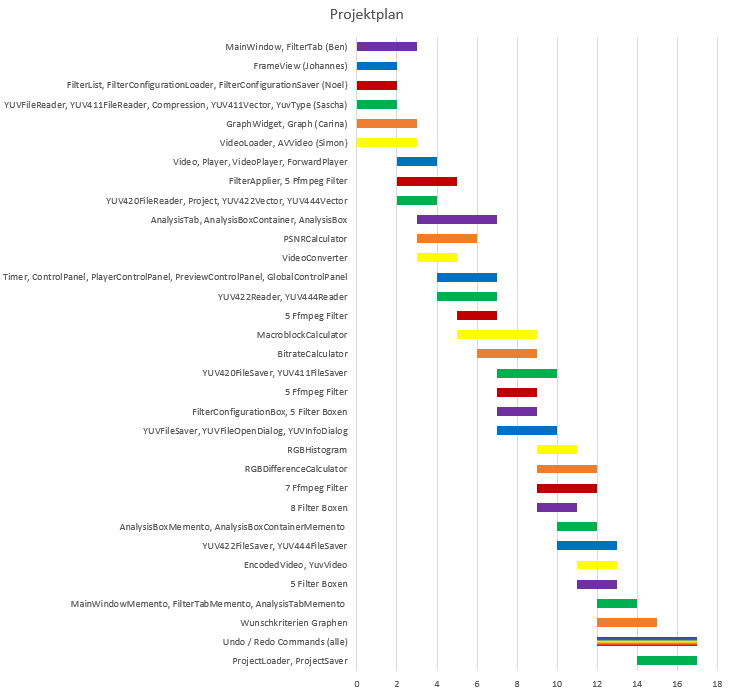
\includegraphics[width=1.0\textwidth]{Pictures/gantt.png}
\caption{Ganttdiagramm der Implementierungsphase}
\end{figure}
\newpage
\subsection{Grobübersicht der Entwurfsänderungen}
In diesem Abschnitt werden die größten Änderungen in den einzelnen Pakten kurz erlätert und begründet.
\subsubsection{Allgemein}
Auch wenn die Änderungen auf den ersten Blick groß und umfrangreich erscheinen, hat sich die grobe Idee, wie die Klassen miteinander kommunizieren und interagieren, nicht gändert.
\paragraph{Smartpointer} Viele Änderung im gesamten Entwurf beziehen sich auf die Benutzung von Smartpointer anstatt von 'nackten' Pointern. Obwohl uns während des Entwurfs schon klar war, dass wir auf Smartpointer setzen werden, hatten wir keine Möglichkeit dies im Klassen diagramm korrekt darzustellen. Hauptproblem war dabei, dass Smartpointer häufig Attribute in den Klassen waren und wir diese Attribute mittels Aggregationen und Kompositionen dargestellt haben. Daher waren diese Aggregationen hinterher nur Pointer und keine Smartpointer.
\paragraph{Abstrakte Klassen} Während der Entwurfsphase war uns nicht bewusst, dass es in C++ nur möglich ist, Objekte von abstrakten Klassen als Pointer zu übergeben. Deshalb mussten vorallem viele Methoden, die einen Filter als Parameter nehmen, geändert werden.
\paragraph{Vergessenes} Ein kleiner Teil der Änderungen sind Attribute, die im Entwurf einfach vergessen wurden. Ein weiterer Faktor war auch, dass beim Ändern einer Klasse andere Klassen, die diese benutzten, nicht korrekt angepasst wurden.
\bigskip
\subsubsection{Utility Paket}
\paragraph{Threading}
Fast alle Änderungen in diesem Packet wurden gemacht, um das  asynchrone Laden und Berrechnen von Videos und Graphen zu ermöglichen. Der Grund, weshalb wir Threading während des Entwurfs nicht mit einbezogen hatte, ist, dass wir nicht genau wussten, wie wir Threads einbinden und das Signalhandling entwerfen sollen.
\bigskip
\subsubsection{Model Paket}
\paragraph{Bessere Schnittstelle} Die meisten Änderungen in diesem Paket wurden gemacht, um das Benutzen der Klassen einfacher zu machen. Teilweise passte die Schnittstelle, aufgrund von Änderungen an anderen Stellen, nicht mehr zu dem, was benötigt wurde. 
\bigskip
\subsubsection{UndoRedo Paket}
Bei den Klassen in diesem Packet hatten wir schon während des Entwurfs große Schwierigkeiten einzuschätzen, was notwendig ist, um eine Aktion wieder rückgängig zu machen. Vorallem da Änderungen an einer Stelle im Entwurf sich sofort auf den entsprechenden Undo-command auswirken, hat dieses Packet schon im Entwurf viele Änderungen erfahren.
\bigskip
\subsubsection{Memento Paket}
\paragraph{Pointer} Bei den Mementos hatten wir ursprünglich die Idee, dass sie die Daten, die sie halten, auch besitzen. Das impliziert, dass jedes mal, wenn ein Memento erstellt wird, viel kopiert wird. Das hat sich vorallem im Hinblick auf die Videos als eher unpracktikabel herrausgestellt. Daher wurden viele Attribute und Parameter zu Pointern gemacht.
\paragraph{Vergessene Daten} Ebenfalls viele Änderungen beziehen sich auf Attribute, die wir einfach vergessen haben anzugeben.
\bigskip
\subsubsection{GUI Paket}
\paragraph{Änderungen an der GUI} In diesem Packet sind,qie zu erwarten, die meisten Änderungen passiert. Das hängt vorallem damit zusammen, dass wir an manchen Stellen die GUI abgändert haben, weil sich Teile des geplanten Aufbaus als zu Umständlich in der Bedienung entpuppt haben, oder einfach nicht ins Gesamtbild passten. Allerdings lösen selbst kleine Änderungen ziemlich große Änderungen am Entwurf aus. Auch das Zusammenspiel der einzelnen GUI-Komponeneten hatten wir nicht richtig durchdacht, weshalb es in diesem Bereich auch etliche Änderungen gab.
\newpage
\subsection{Änderungen an der GUI}
Es gab keine großen struktuellen Änderungen an der GUI. Das Look and Feel unterscheidet sich aber trotzdem deutlich von der erstellten Beispieloberfläche im Pflichtenheft. Sieht dort alles noch recht unorganisiert und gestaucht aus, setzt die fertige Oberfläche auf weiche Kanten, deutliche Übergänge zwischen den einzelnen Elementen und ein allgemein stimmiges Gesamtbild. In den folgenden Abschnitten werden die konkreten Unterschiede beschrieben und erläutert.
\newpage
\subsubsection{YuvFileOpen Dialog}
\bigskip
\begin{figure}[ht]
\centering
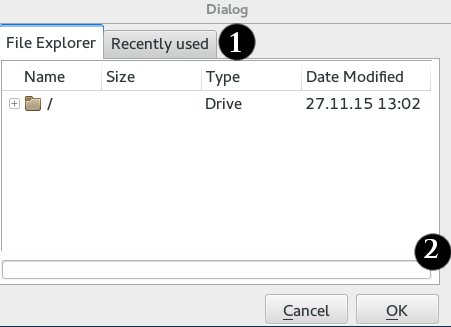
\includegraphics[width=0.7\textwidth]{Pictures/fileopenalt.jpg}
\caption{YuvFileOpenDialog aus dem Pflichtenheft}
\end{figure}
\begin{figure}[ht]
\centering
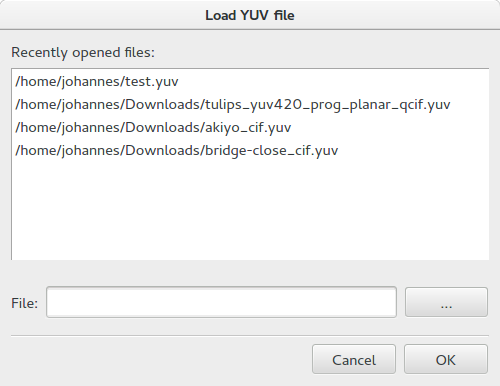
\includegraphics[width=0.7\textwidth]{Pictures/fileopenneu.png}
\caption{YuvFileOpenDialog im fertigen Pogramm}
\end{figure}
Die Tabs wurden zu einem verschmolzen und der Dateiexplorer ganz entfernt. Dieser ist nun über den Button (...) erreichbar. Wir haben uns für diese Änderung entschieden, da es nicht ohne weiteres möglich war, einen Dateiexplorer direkt einzubinden und haben daher eine einfachere Variante gewählt.
\newpage
\subsubsection{YuvFileInfo Dialog}
\bigskip
\begin{figure}[ht]
\centering
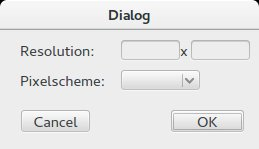
\includegraphics[width=0.5\textwidth]{Pictures/fileinfoalt.jpg}
\caption{YuvFileInfoDialog aus dem Pflichtenheft}
\end{figure}
\begin{figure}[ht]
\centering
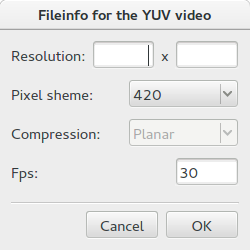
\includegraphics[width=0.5\textwidth]{Pictures/fileinfoneu.png}
\caption{YuvFileInfoDialog im fertigen Pogramm}
\end{figure}
Neben kleinen Umordungen der Elemente sind außerdem noch weitere Eingabefelder für die Kompression und die Fps des Videos hinzugekommen. Die Kompression ist hinzugekommen, da wir jedes Pixelformat, außer 420, nun auch planar als auch packed unterstützen. Das Fps Feld ist dazu gekommen, um es dem Nutzer zu ermöglichen, Videos mit einer beliebigen Fps abzuspielen.
\newpage
\subsubsection{Filtertab}
\bigskip
\begin{figure}[ht]
\centering
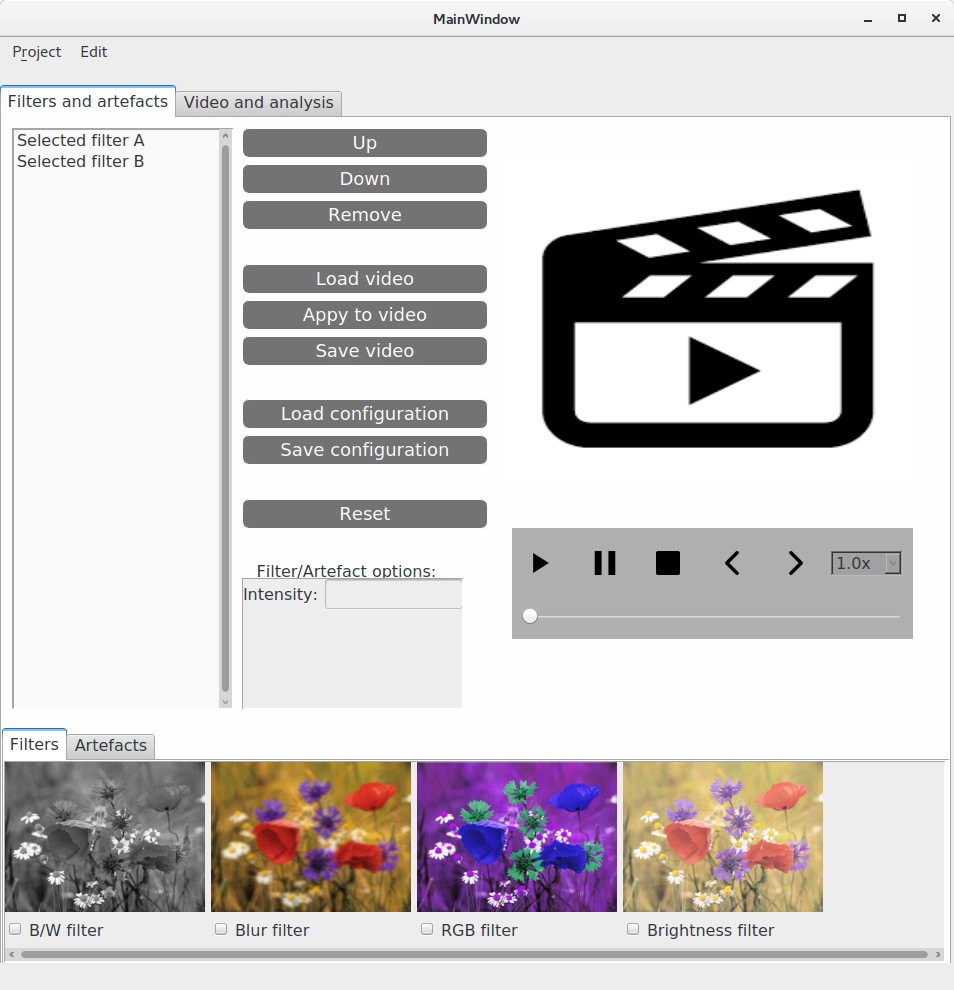
\includegraphics[width=0.9\textwidth]{Pictures/filtertabalt.png}
\caption{Filtertab aus dem Pflichtenheft}
\end{figure}
\begin{figure}[ht]
\centering
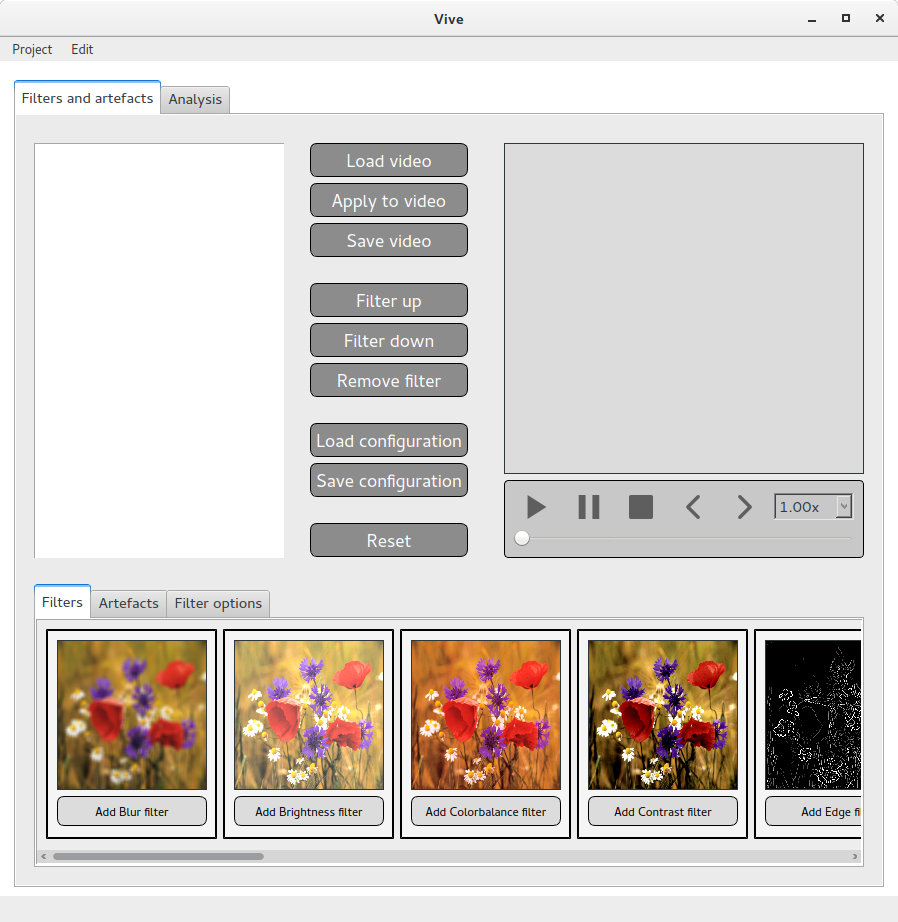
\includegraphics[width=0.9\textwidth]{Pictures/filtertabneu.png}
\caption{Filtertab im fertigen Pogramm}
\end{figure}
Im Filtertab gab es keine großartigen Anpassungen. Der deutlichste Unterschied ist, dass die Oberfläche im fertigen Programm farblich besser abgestimmt und wesentlich ansprechender ist. Einige kleine Änderungen gab es aber dennoch. Zum einem wurden die Checkboxen bei der Filterauswahl durch Buttons ersetzt, einfach um es dem Nutzer zu ermöglichen, einen Filter mehr als einmal anzuwenden. Die zweite und letzt Änderung am Filtertab, ist, dass die Filteroptionen einen eigenen Tab bekommen haben und nicht mehr mitten in der GUI hängen. Diese Änderung wurde rein aus Platzgründen gemacht.
\newpage
\hfill
\newpage
\subsubsection{Analyisistab}
\bigskip
\begin{figure}[ht]
\centering
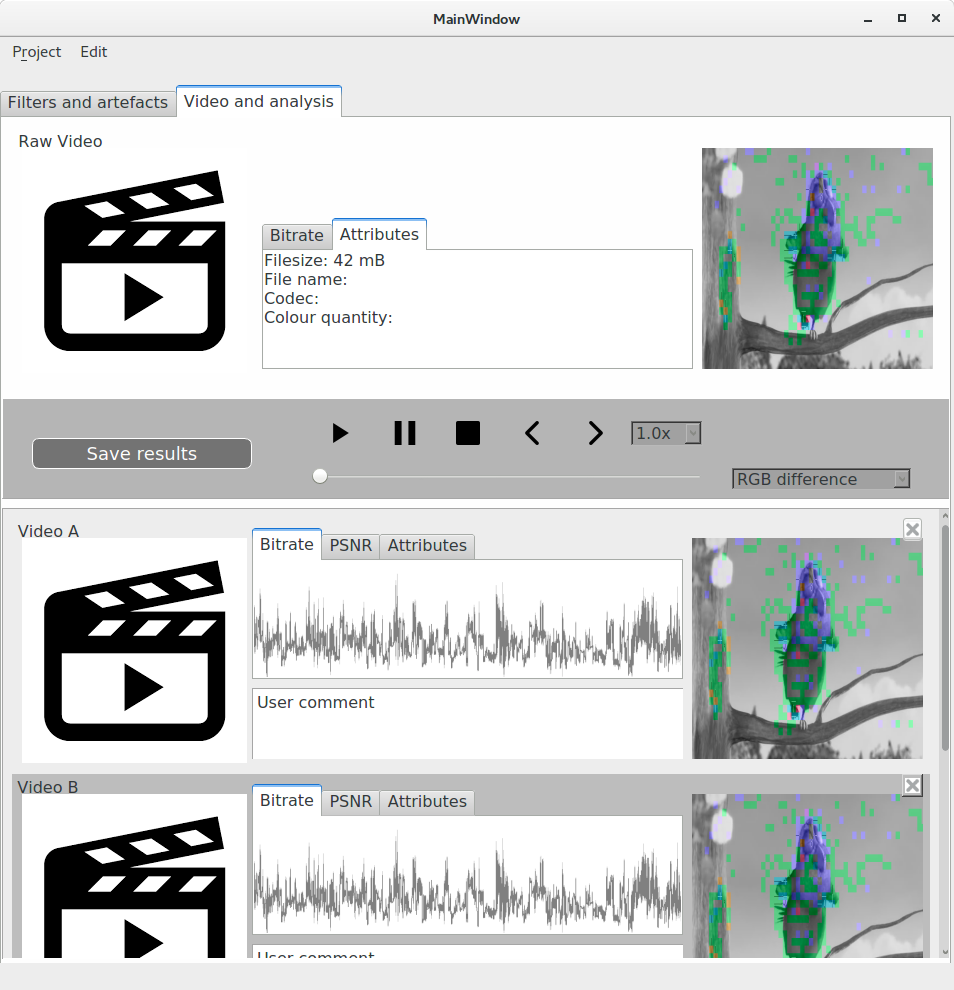
\includegraphics[width=0.9\textwidth]{Pictures/analysistabalt.png}
\caption{Analysistab aus dem Pflichtenheft}
\end{figure}
\begin{figure}[ht]
\centering
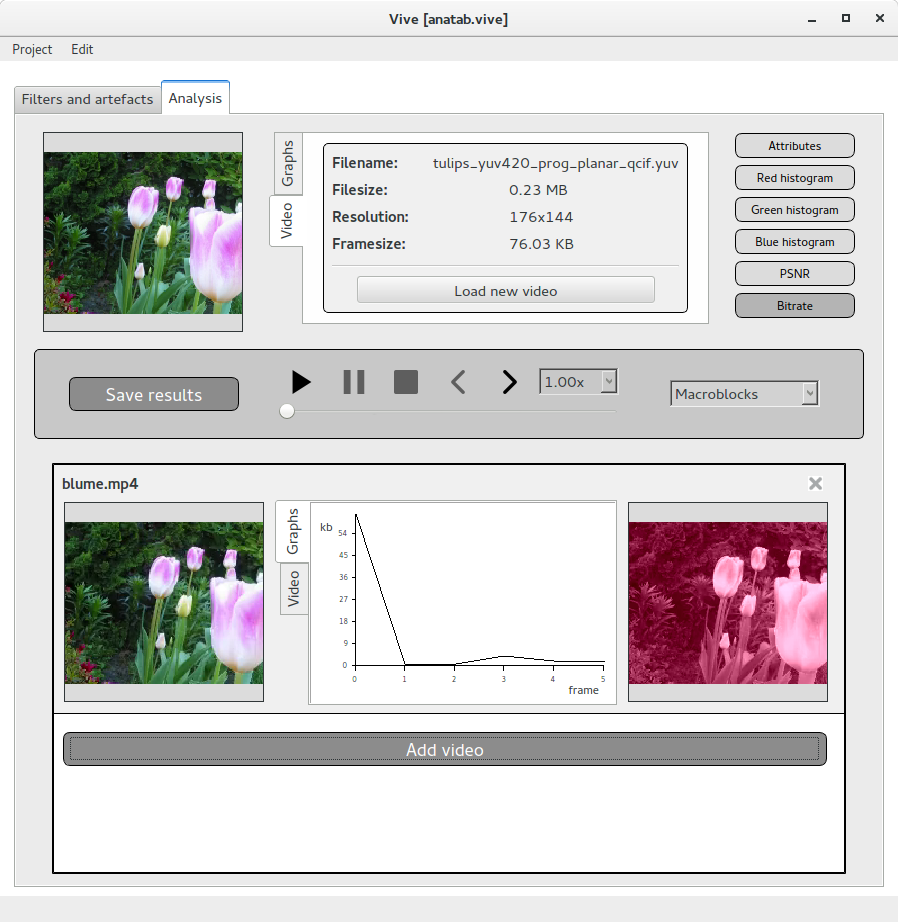
\includegraphics[width=0.9\textwidth]{Pictures/analysistabneu.png}
\caption{Analysistab im fertigen Pogramm}
\end{figure}
Ähnlich wie beim Filtertab ist auch hier die größte Änderung die optische Verschönerung des Gesamtbildes. Die einzige wichtige Veränderung, die passiert ist, ist, dass bei den encodeden Videos statt der einzelnen Tabs nun Buttons neben das Rohvideo gesetzt wurde, mit denen man auswählen kann, welcher Graph für alle Videos angezeigt werden soll. Diese Änderung erhöht den Komfort bei der Analyses immens, da nun nicht immer bei jedem Video einzeln der entsprechende Graph ausgeählt werden muss, um diese zu vergleichen.
\newpage
\hfill
\newpage
\subsection{Entfernte Funktionalität}
\bigskip
\paragraph{Ergebnisse speichern beim Speichern des Projektes} Diese Funktionalität war weniger ein Implementierungstechnisches Problem als eine schlechte Entscheidung. Im Pflichtenheft hatten wir geplant, dass berechnete Videos und Graphen beim Projekt speichern mit abgespeichert werden und später, wenn das Projekt wieder geladen wird, auch wieder geladen werden. Allerdings geht das Neuberechnen dieser schneller, als das komplette Einlesen der Dateien. Deshalb wurde diese Funktionalität entfernt und berechnete Videos und Graphen können nur noch separat über die Ergebnisse speichern Funktionalität abgespeichert werden.
\paragraph{Blenden Filter} Dieser Filter sollte bewirken, dass das Video entweder von einem schwarzen Bild aus einblendet oder auf ein schwarzes Bild ausblendet. Allerdings steht dieser Filter im Konflikt mit der Filtervorschau, da das Video komplett berechnet werden müsste, um die Vorschau korrekt darzustellen und wurde daher entfernt.
\paragraph{Zoom Filter} Bei diesem Filter sind wir auf ein Bug in der libavfilter Bibliothek gestoßen, der das Bild bei der Ausgabe falsch skalierte. Um diesen Bug zu umgehen, hätten wir einige unschöne Änderungen am Entwurf machen müssen und haben den Filter daher nicht implementiert.
\paragraph{Anzahl der Farben in encodierten Videos} Die Anzahl der Farben im Video sollte als Attribut bei den encodierten Videos angezeigt werden. Allerdings gibt es keinen effizienten Weg, diese Zahl zu berechnen. Allein um während der Berechnung zu speichern, welche Farbe bereits verwendet wurde, wären ca. 66 MB Arbeitspeicher notwendig, geschweige denn der CPU-Leistung. Daher steht der Aufwand dieses Attributs in keinem Verhältnis zu seiner Wichtigkeit und wurde daher entfernt.
\newpage
\subsection{Zusätzlich implementierte Funtionalität}
\bigskip
\paragraph{Filter mehr als einmal anwenden} Im Pflichtenheft war vorgesehen, dass ein Filter nur maximal einmal auf ein Video angewendet werden kann. Da diese Einschränkung implementierungstechnisch jedoch mehr Aufwand gewesen wäre, haben wir sie weggelassen.
\paragraph{Attribute für das Rohvideo im Analysistab} Folgende Attribute werden für das Rohvideo angezeigt: Dateiname, Dateigröße, Auflösung und die Größe eines Frames im Arbeitsspeicher.
\paragraph{Zusätzliches Attribut für encodierte Videos} Folgendes Attribut wird zusatzlich für encodierte Videos angezeigt: Durchschnittliche Bitrate.
\paragraph{Bei Klick auf Bitrategraph im Video springen} Diese Funktionalität wurde nur für den Psnrgraphen spezifiziert. Allerdings war es kein großer Aufwand, diese Funktionalität auch dem Bitrategraphen zu geben, weshalb man nun auch bei einem Klick auf den Bitrategraphen im Video springen kann.
\paragraph{Anzeigen von Motionvektoren} Zusätzlich zu den Macroblöcken werden im selben Video auch noch die Motiovektoren. Der Grund für diese Änderung ist allerdings ein Bug in der libavcodec Bibliothek.
\paragraph{Zusätzliche Angaben im YuvFileInfoDialog} Folgende Zusätzliche Angaben können gemacht werden: Fps, Kompression.
\newpage
\section{Testüberdeckung}
Während der Implementierung haben wir bereits damit begonnen, Testcode zu schreiben.
\paragraph{Getestete Klassen} Es sind Unit Tests für alle Klassen der Packete Model und Memento vorhanden, sowie für die Klasse VideoConverter aus dem Packet Utility. Das ergibt eine insgesamte Anzahl von 35 Klassen.

\paragraph{Testüberdeckung} Alle Testfälle ergeben eine Zeilenanzahl von 1900, was einer Testüberdeckung von 23\% entsprichht.


\end{document}